% !Mode:: "TeX:UTF-8"
\chapter{插图}
\label{chap:figures}

插图主要涉及到:单个居中图形;两个并排图形;两个以上的并排或者堆叠的图形;图题;图形的引用;

\section{单个居中图形}\label{section2-1}

大多数情况下,需要插入的图形是单个的时候可以使用如下环境:

\begin{verbatim}
\begin{figure}[hptb!]
 \centering\small
 
\includegraphics[width=0.6\textwidth]{ysulogo}
 \FigureBiCaption{单个居中图形}
 {A single center graphics A single center graphics}\label{ysulogo}%\vspace{0.3em}
\end{figure}

或者

\begin{figure}[hptb!]
 \centering\small
 
\includegraphics[width=0.6\textwidth]{ysulogo}
 \caption{单个居中图形\label{ysulogo}}\vspace{0.3em}
 \begin{minipage}[t]{0.9\textwidth}
 \centering
 {Fig.  \ref{ysulogo} A single center graphics}
 \end{minipage}
\end{figure}
\end{verbatim}
其中的参数“[width=$\backslash$textwidth]”指定图形的宽度0.6倍页宽。两种方式都可以达到最后的效果如图 \ref{ysulogo}所示。个人推荐第一种方式。
\begin{figure}[hptb!]
 \centering\small
 
\includegraphics[width=0.6\textwidth]{ysulogo}
 \FigureBiCaption{单个居中图形}
 {A single center graphics A single center graphics }\label{ysulogo} 
\end{figure}


\section{两个并排图形}\label{section2-2}
下列代码在文中插入两个并排的图形。它使用了一个称作minipage
的环境。在同一行插入两个并排的minipage,每个minipage包含一
个图形。图中minipage的参数“[0.5$\backslash$linewidth]”指定minipage
的宽度是当前正文页面的0.5倍(一半)。而插图命令中的参数
“[width=$\backslash$textwidth]”则是指定插图的宽度为当前minipage的宽
度。如果这个插图命令是在minipage环境外边的话,参数中的
“$\backslash$textwidth”的宽度为当前正文页面的宽度。
\begin{verbatim}
\begin{figure}[htbp!]
\centering
\subfigure{\label{subfigure1}}\addtocounter{subfigure}{-2}
\subfigure[The 1st subfigure caption]{\subfigure[第1个子图标题]
{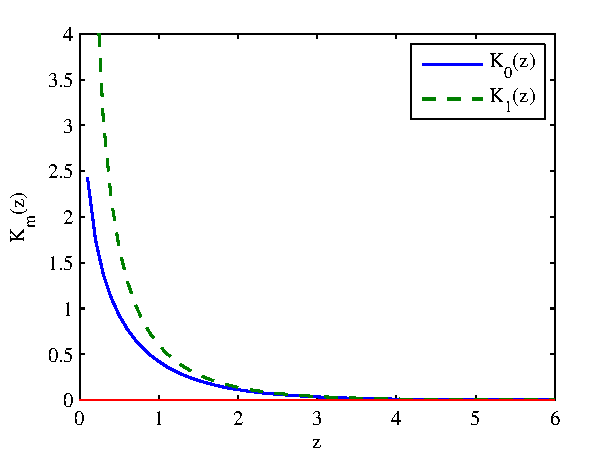
\includegraphics[width=0.46\textwidth]{chp-2_bessel_k}}}%%%%%%%第1个子图
\subfigure{\label{subfigure2}}\addtocounter{subfigure}{-2}
\subfigure[The 2nd subfigure caption]{\subfigure[第2个子图标题]
{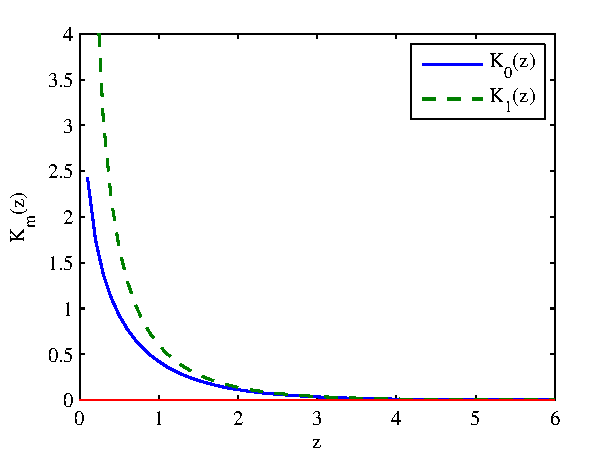
\includegraphics[width=0.46\textwidth]{chp-2_bessel_k}}}%%%%%%%第2个子图
\FigureBiCaption{中文总标题}{The total caption\label{Figure-all}}
\end{figure}

或者

\begin{figure}[hptb!]
  \centering\small
  \begin{minipage}[t]{0.5\linewidth}
    \centering
    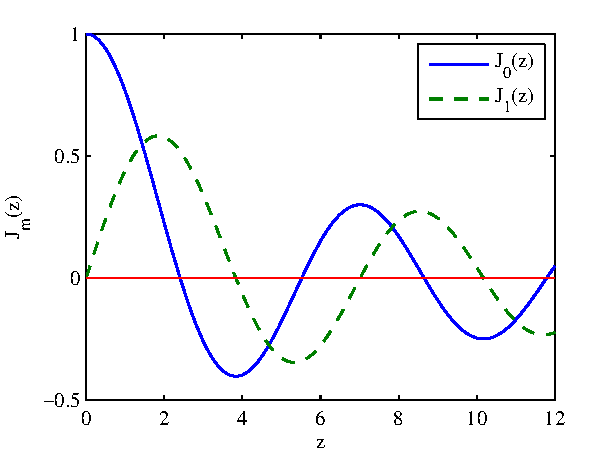
\includegraphics[width=\textwidth]{chp-2_bessel_j}
    (a) 子图a图题\\[0.3em]
    (a) Subfigure a
  \end{minipage}%
  \begin{minipage}[t]{0.5\textwidth}
    \centering
    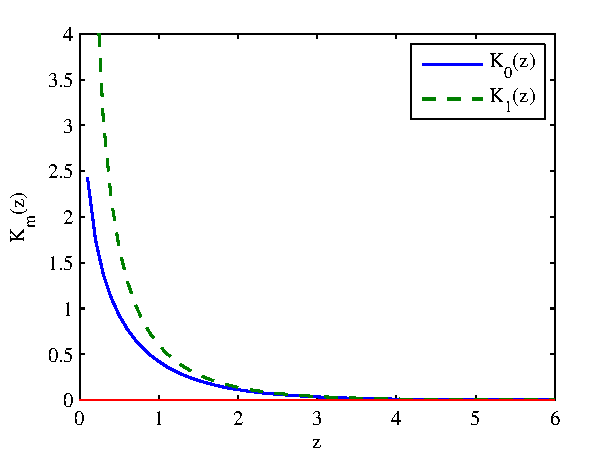
\includegraphics[width=\textwidth]{chp-2_bessel_k}
    (b) 子图b图题\\[0.3em]
    (b) Subfigure b
  \end{minipage}
  \FigureBiCaption{两个并排图形}{Two coordinate graphics}\label{fig-dbfig}
 \end{figure}

或者

\begin{figure}[hptb!]
  \centering\small
  \begin{minipage}[t]{0.5\linewidth}
    \centering
    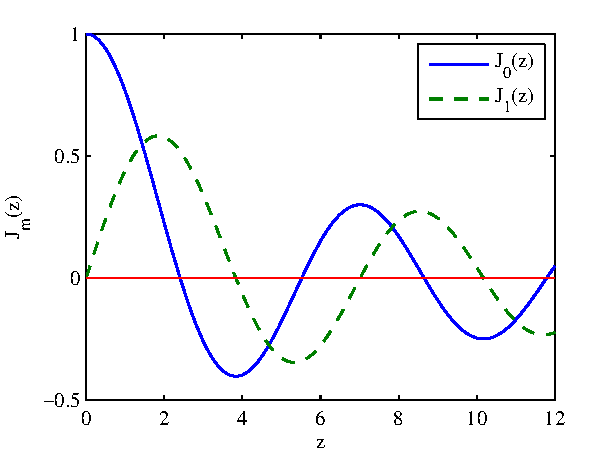
\includegraphics[width=\textwidth]{chp-2_bessel_j}
    (a) 子图a图题\\[0.3em]
    (a) Subfigure a
  \end{minipage}%
  \begin{minipage}[t]{0.5\textwidth}
    \centering
    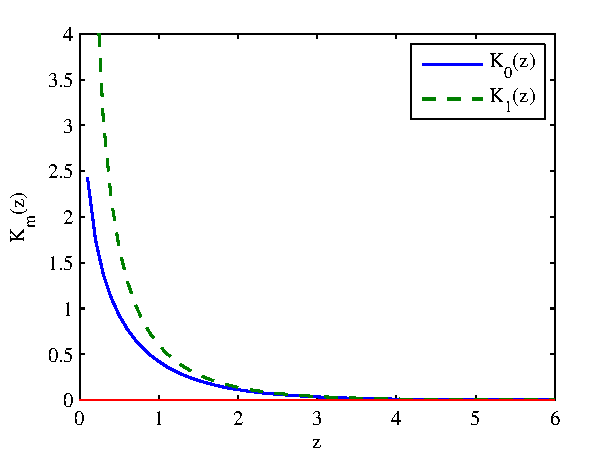
\includegraphics[width=\textwidth]{chp-2_bessel_k}
    (b) 子图b图题\\[0.3em]
    (b) Subfigure b
  \end{minipage}
    \caption{两个并排图形\label{fig-dbfig}}
    \vspace{0.3em}
 \begin{minipage}[t]{0.9\textwidth}
 \centering
 {Fig.  \ref{fig-dbfig} Two coordinate graphics}
 \end{minipage}
 \end{figure}
\end{verbatim}
最终结果如图 \ref{fig-dbfig}所示。
\begin{figure}[htbp!]
\centering
\subfigure{\label{subfigure1}}\addtocounter{subfigure}{-2}
\subfigure[The 1st subfigure caption]{\subfigure[第1个子图标题]
{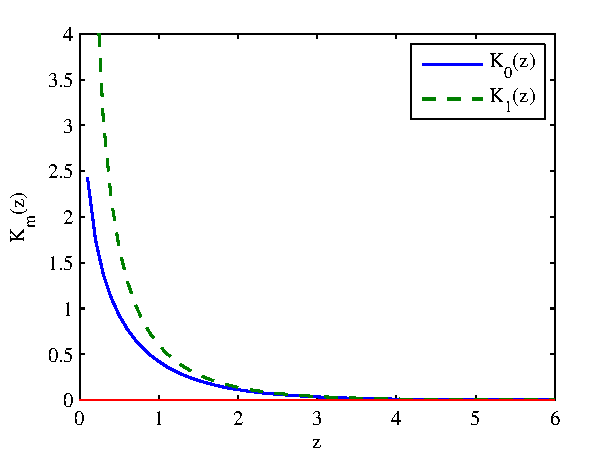
\includegraphics[width=0.46\textwidth]{chp-2_bessel_k}}}%%%%%%%第1个子图
\subfigure{\label{subfigure2}}\addtocounter{subfigure}{-2}
\subfigure[The 2nd subfigure caption]{\subfigure[第2个子图标题]
{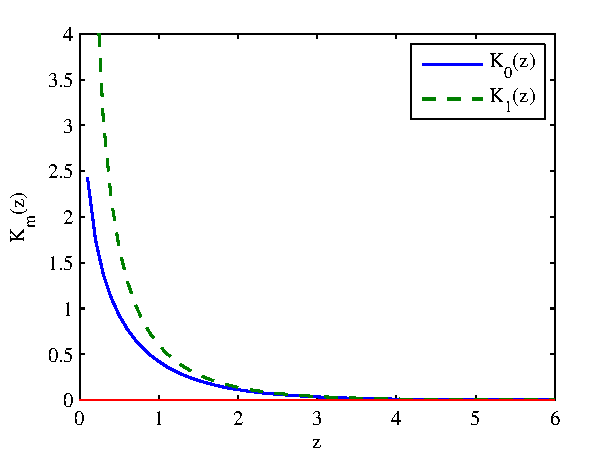
\includegraphics[width=0.46\textwidth]{chp-2_bessel_k}}}%%%%%%%第2个子图
\FigureBiCaption{中文总标题}{The total caption\label{Figure-alll}}
\end{figure}

\begin{figure}[hptb!]
  \centering\small
  \begin{minipage}[t]{0.5\linewidth}
    \centering
    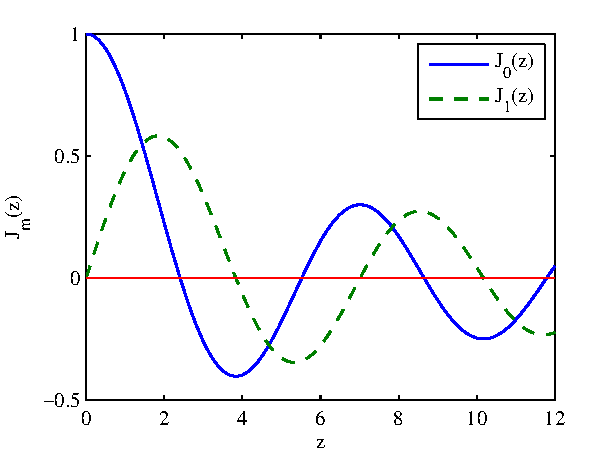
\includegraphics[width=\textwidth]{chp-2_bessel_j}
    (a) 子图a图题\\[0.3em]
    (a) Subfigure a Subfigure a
  \end{minipage}%
  \begin{minipage}[t]{0.5\textwidth}
    \centering
    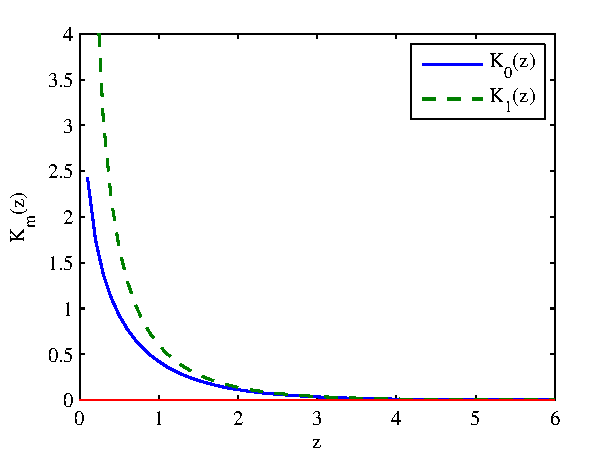
\includegraphics[width=\textwidth]{chp-2_bessel_k}
    (b) 子图b图题\\[0.3em]
    (b) Subfigure b Subfigure b
  \end{minipage}
  \FigureBiCaption{两个并排图形}{Two coordinate graphics}\label{fig-dbfig}
 \end{figure}



\section{两个以上的并排或者堆叠的图形}\label{section2-3}
同样是使用minipage的方法,只不过排列的方式不同。例如4幅堆叠排列的图形。
\begin{verbatim}
\begin{figure}[htbp!]
\centering
\subfigure{\label{subfigure1}}\addtocounter{subfigure}{-2}
\subfigure[The 1st subfigure caption]{\subfigure[第1个子图标题]
{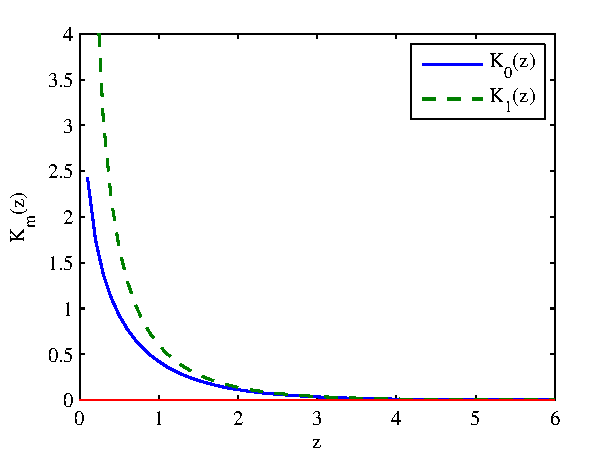
\includegraphics[width=0.46\textwidth]{chp-2_bessel_k}}}%%%%%%%第1个子图
\subfigure{\label{subfigure2}}\addtocounter{subfigure}{-2}
\subfigure[The 2nd subfigure caption]{\subfigure[第2个子图标题]
{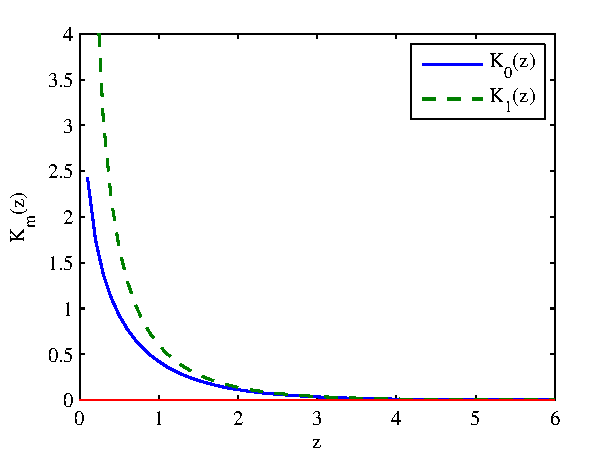
\includegraphics[width=0.46\textwidth]{chp-2_bessel_k}}}\\[-1.5em]%%%%%%%第2个子图
\subfigure{\label{subfigure1}}\addtocounter{subfigure}{-2}
\subfigure[The 3rd subfigure caption]{\subfigure[第3个子图标题]
{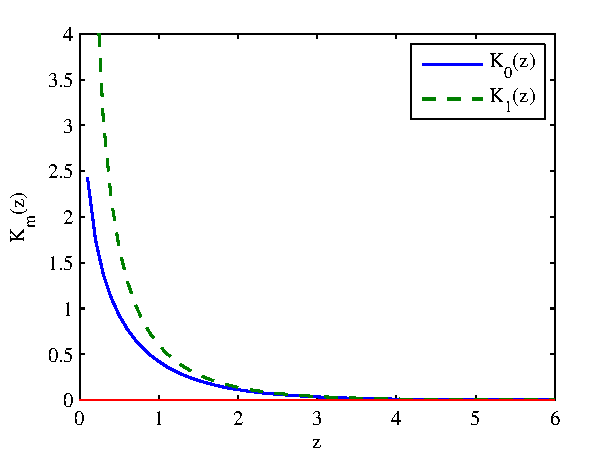
\includegraphics[width=0.46\textwidth]{chp-2_bessel_k}}}%%%%%%%第3个子图
\subfigure{\label{subfigure4}}\addtocounter{subfigure}{-2}
\subfigure[The 4th subfigure caption]{\subfigure[第4个子图标题]
{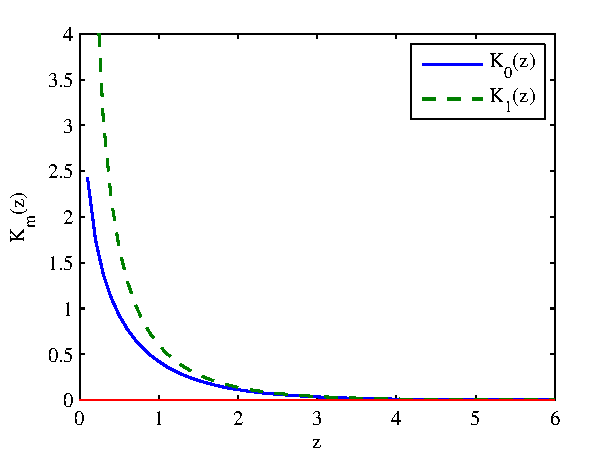
\includegraphics[width=0.46\textwidth]{chp-2_bessel_k}}}%%%%%%%第4个子图\\
\FigureBiCaption{中文总标题}{The total caption\label{Figure-all}}
\end{figure}

或者

\begin{figure}[hptb!]
  \centering\small
  \begin{minipage}[t]{0.5\linewidth}
    \centering
    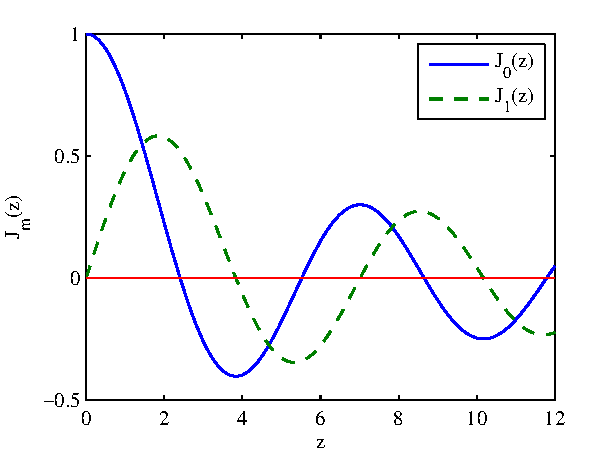
\includegraphics[width=\textwidth]{chp-2_bessel_j}
    (a) 子图a图题\\[0.3em]
    (a) Subfigure a
  \end{minipage}%
  \begin{minipage}[t]{0.5\textwidth}
    \centering
    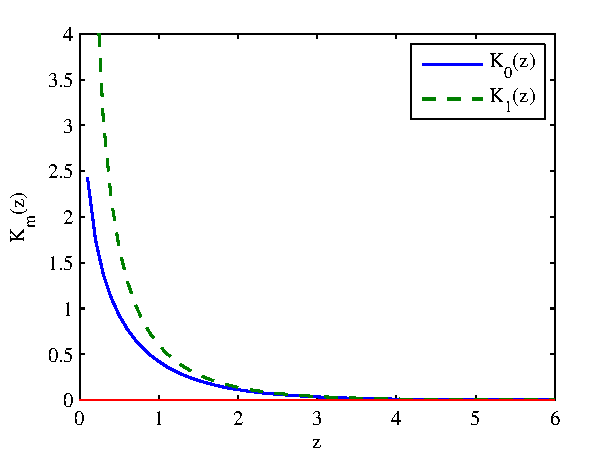
\includegraphics[width=\textwidth]{chp-2_bessel_k}
    (b) 子图b图题\\[0.3em]
    (b) Subfigure b
  \end{minipage}  \\
  \begin{minipage}[t]{0.5\textwidth}
    \centering
    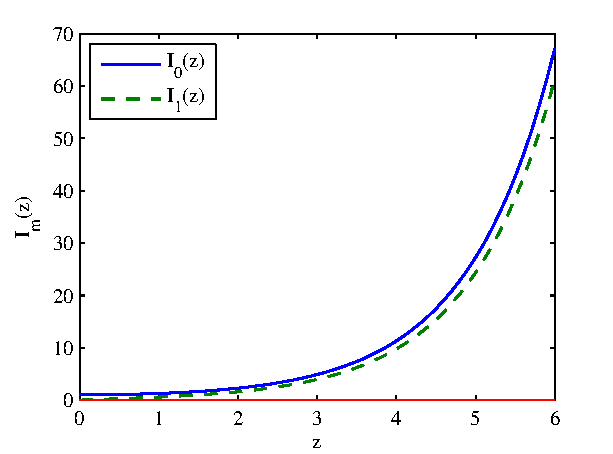
\includegraphics[width=\textwidth]{chp-2_bessel_i}
    (c) 子图c图题\\[0.3em]
    (c) Subfigure c
  \end{minipage}%
  \begin{minipage}[t]{0.5\textwidth}
    \centering
    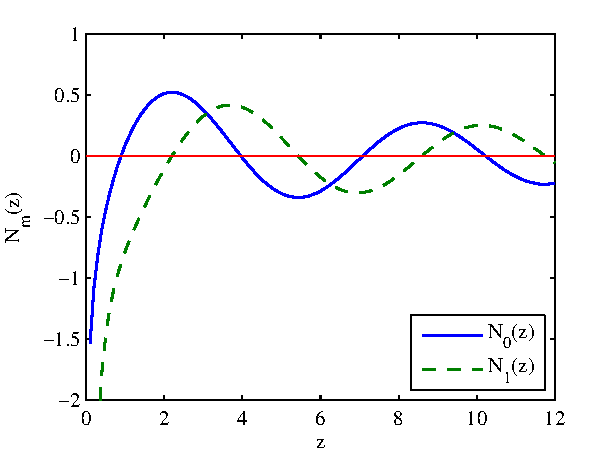
\includegraphics[width=\textwidth]{chp-2_bessel_n}
    (d) 子图d图题\\[0.3em]
    (d) Subfigure d
  \end{minipage}
  \FigureBiCaption{贝塞尔函数}{Bessel function}\label{fig-bessel-function}
\end{figure}
\end{verbatim}
注意其中与一对并排图形不同的地方,加入了换行命令“$\backslash\backslash$”。
最终效果如图 \ref{fig-bessel-function}所示。
\begin{figure}[htbp!]
\centering\small
\subfigure{\label{subfigure11}}\addtocounter{subfigure}{-2}
\subfigure[The 1st subfigure caption]{\subfigure[第1个子图标题]
{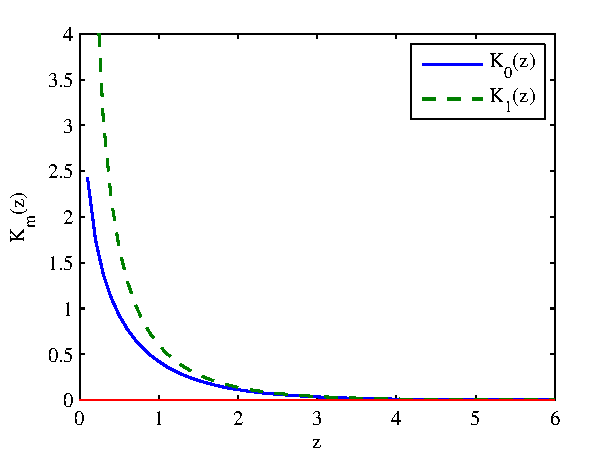
\includegraphics[width=0.46\textwidth]{chp-2_bessel_k}}}%%%%%%%第1个子图
\subfigure{\label{subfigure22}}\addtocounter{subfigure}{-2}
\subfigure[The 2nd subfigure caption]{\subfigure[第2个子图标题]
{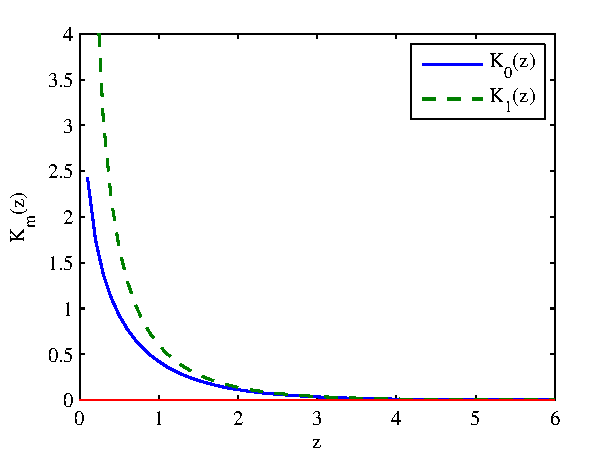
\includegraphics[width=0.46\textwidth]{chp-2_bessel_k}}}\\[-1.5em]%%%%%%%第2个子图
\subfigure{\label{subfigure3}}\addtocounter{subfigure}{-2}
\subfigure[The 3rd subfigure captionThe 3rd subfigure caption]{\subfigure[第3个子图标题第3个子图标题]
{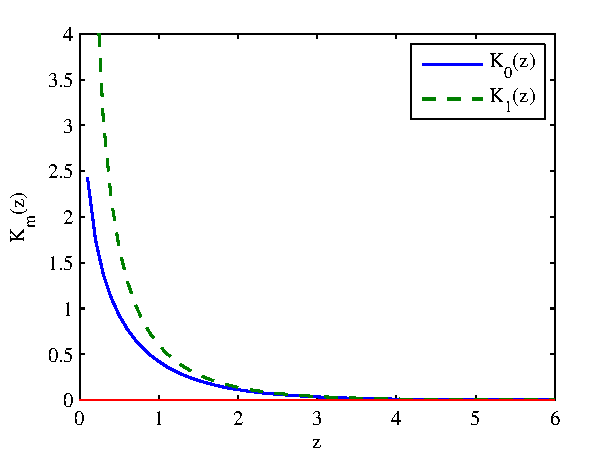
\includegraphics[width=0.46\textwidth]{chp-2_bessel_k}}}%%%%%%%第3个子图
\subfigure{\label{subfigure4}}\addtocounter{subfigure}{-2}
\subfigure[The 4th subfigure captionThe 4th subfigure caption]{\subfigure[第4个子图标题第4个子图标题]
{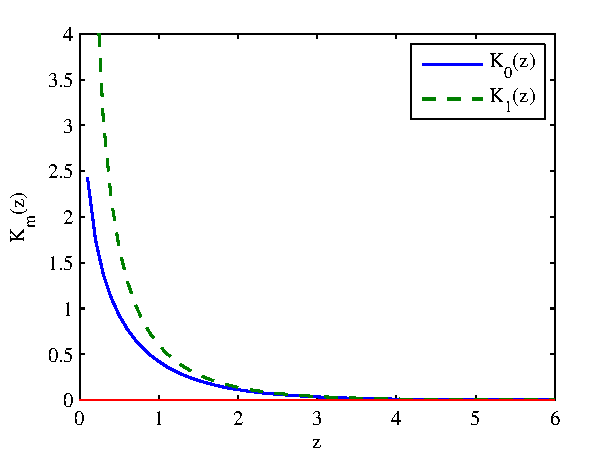
\includegraphics[width=0.46\textwidth]{chp-2_bessel_k}}}%%%%%%%第4个子图\\
\FigureBiCaption{中文总标题}{The total caption\label{Figure-all}}
\end{figure}
\begin{figure}[hptb!]
  \centering\small
  \begin{minipage}[t]{0.5\linewidth}
    \centering
    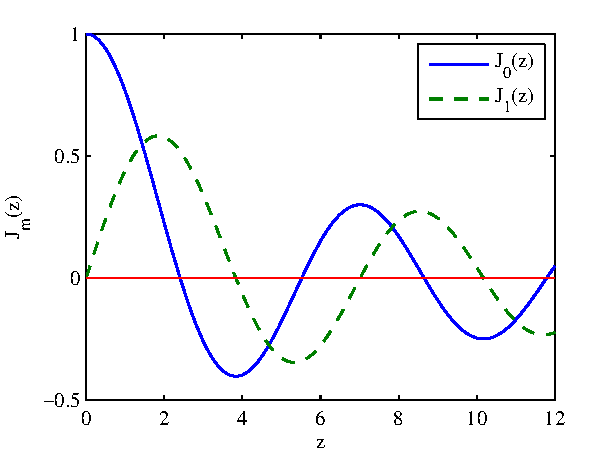
\includegraphics[width=\textwidth]{chp-2_bessel_j}
    (a) 子图a图题\\[0.3em]
    (a) Subfigure a
  \end{minipage}%
  \begin{minipage}[t]{0.5\textwidth}
    \centering
    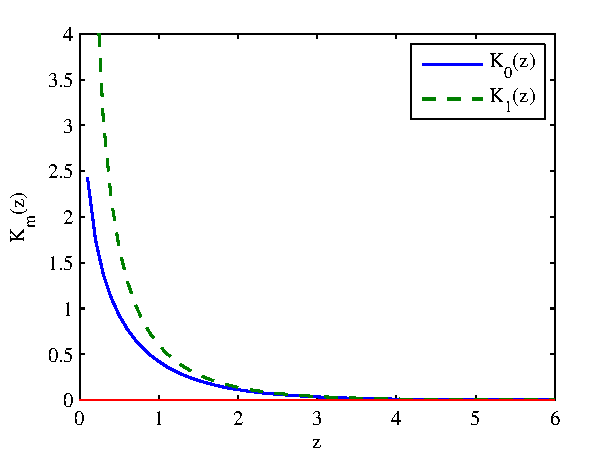
\includegraphics[width=\textwidth]{chp-2_bessel_k}
    (b) 子图b图题\\[0.3em]
    (b) Subfigure b
  \end{minipage}  \\
  \begin{minipage}[t]{0.5\textwidth}
    \centering
    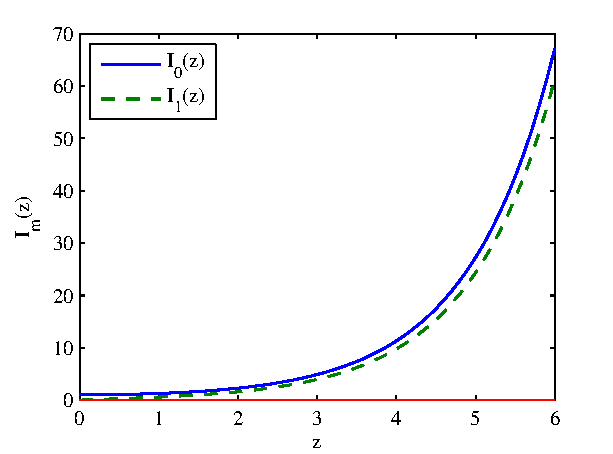
\includegraphics[width=\textwidth]{chp-2_bessel_i}
    (c) 子图c图题\\[0.3em]
    (c) Subfigure c
  \end{minipage}%
  \begin{minipage}[t]{0.5\textwidth}
    \centering
    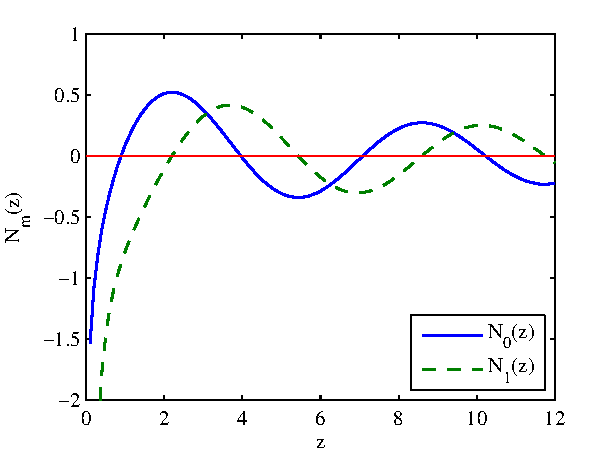
\includegraphics[width=\textwidth]{chp-2_bessel_n}
    (d) 子图d图题\\[0.3em]
    (d) Subfigure d
  \end{minipage}
  \FigureBiCaption{贝塞尔函数}{Bessel function} \label{fig-bessel-function}
\end{figure}

其它类似的多个图形并排或者堆叠均可以灵活的运用minipage照猫画虎获得。

\section{图题}\label{section2-4}
其实上边的例子中已经包含了图题的引用命令\verb|\FigureBiCaption|或命令\verb|\caption|两种方式,个人推荐使用第一种。
例如图 \ref{fig-bessel-function}中:
\begin{verbatim}
  \FigureBiCaption{贝塞尔函数}{Bessel function}\label{fig-bessel-function}
或
  \caption{贝塞尔函数\label{fig-bessel-function}}\vspace{0.3em}
  {Fig.  \ref{fig-bessel-function} Bessel function}
\end{verbatim}
为当前的图形添加中文图题“贝塞尔函数”,及英文图题“Bessel function”。同时添加标签“fig-bessel-function”。对图形的引用就是通过标签来实现的。

\section{图形的引用}\label{section2-5}
在已知图形的标签的基础之上,通过命令:
\begin{verbatim}
 \ref{label}
\end{verbatim}
来引用标签为“label”的图形。\LaTeX 会自动将其替换为图形的编号。例如:
\begin{verbatim}
贝塞尔函数的图形如图 \ref{fig-bessel-function}所示。
\end{verbatim}
的效果如下:\\
贝塞尔函数的图形如图 \ref{fig-bessel-function}所示。

\section{本章小结}\label{section2-6}
注意!从第二章开始应有``本章小结",主要总结本章所做的主要研究工作,研究成果等内容!!!

%
